\documentclass[tikz,border=10pt]{standalone}
\begin{document}
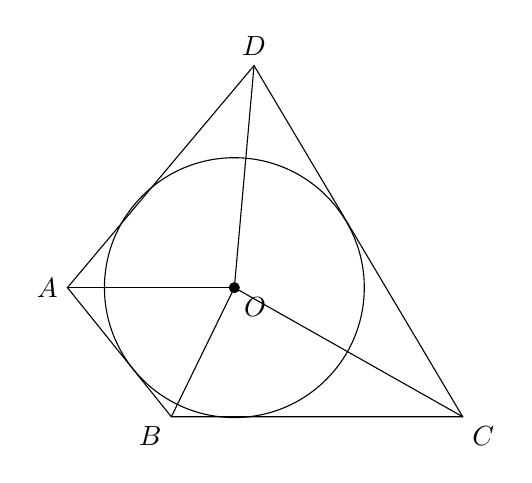
\begin{tikzpicture}
  \coordinate (A) at (0.68,-3.48);
  \coordinate (B) at (2.00,-5.12);
  \coordinate (C) at (5.70,-5.12);
  \coordinate (D) at (3.05,-0.66);
  \coordinate (O) at (2.80,-3.48);

  \draw (A) -- (B) -- (C) -- (D) -- cycle;
  \draw (O) circle (1.65);
  \draw (A) -- (O);
  \draw (B) -- (O);
  \draw (C) -- (O);
  \draw (D) -- (O);
  \fill (O) circle (2pt);

  \node[left] at (A) {$A$};
  \node[below left] at (B) {$B$};
  \node[below right] at (C) {$C$};
  \node[above] at (D) {$D$};
  \node[below right] at (O) {$O$};
\end{tikzpicture}
\end{document}
